\chapter{System Overview}

\section{Architectual structure}

\begin{figure}[h!]
    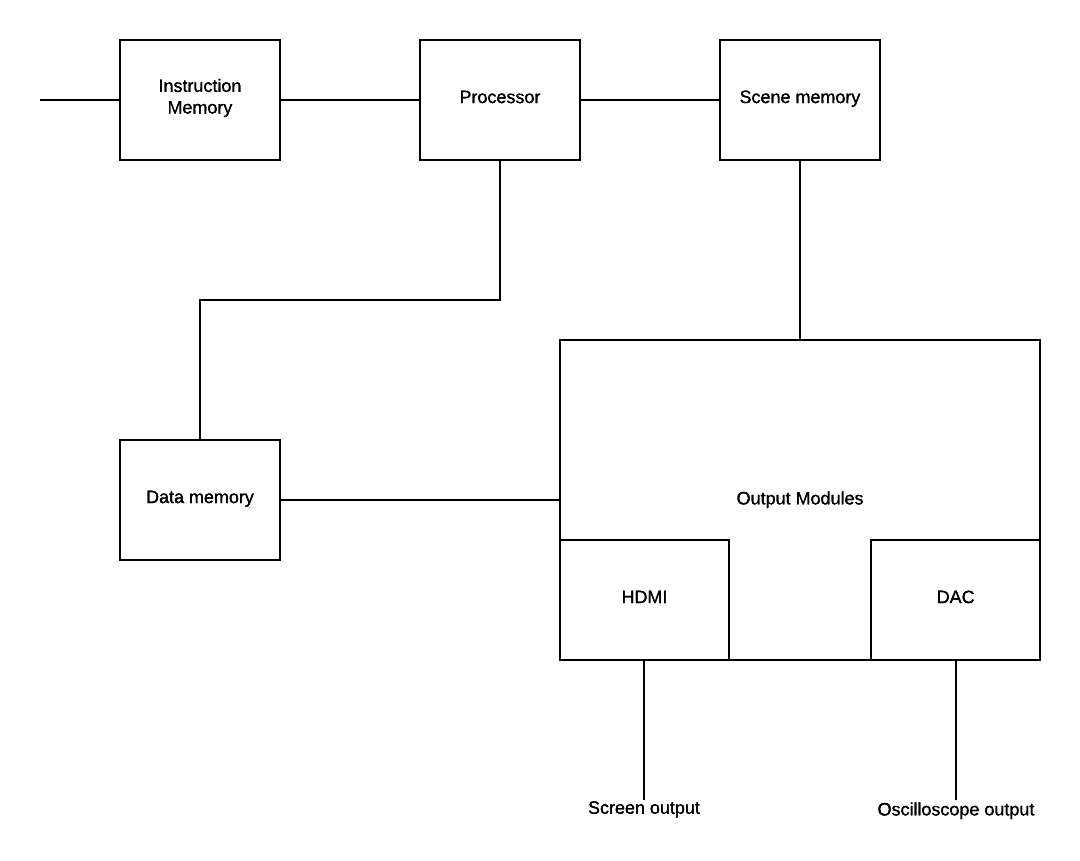
\includegraphics[width=\linewidth]{images/system-overview.png}
    \caption{A logical overview of the \vthreek architecture}
    \label{fig:system-overview}
\end{figure}

Figure \ref{fig:system-overview} shows how the major building blocks of the \vthreek architecture come together on a conceptual level.
Separation of instruction and data memory makes it a Harvard-like architecture.
The processor reads from instruction memory, executes instructions and adds/updates vector primitives in the scene memory.
Preprocessing these primitives for output is done by the output modules.
For the HDMI output, this involves rasterizing each primitive and maintaining a framebuffer.
The oscilloscope output is generated by serializing primitives onto two DACs.
